\documentclass[11pt]{article}
\usepackage[margin=1in]{geometry}
\usepackage[T1]{fontenc}
\usepackage[utf8]{inputenc}
\usepackage{booktabs,graphicx,amsmath,enumitem,url}
\usepackage[dvipsnames]{xcolor}
\usepackage[hidelinks]{hyperref}

% numbers.tex is GENERATED by eval/make_report.py from real run results.
\newcommand{\resultModel}{ollama:llama3.2:3b}
\newcommand{\resultJudge}{ollama:llama3.2:3b}
\newcommand{\resultDate}{2026-10-20}
\newcommand{\nAttack}{245}
\newcommand{\nBenign}{154}
\newcommand{\nTrain}{406}
\newcommand{\asrBase}{10.6}
\newcommand{\asrStruct}{11.8}
\newcommand{\asrRules}{1.6}
\newcommand{\fprRules}{1.9}
\newcommand{\asrClf}{2.4}
\newcommand{\fprClf}{1.9}
\newcommand{\asrJudge}{6.5}
\newcommand{\fprJudge}{0.0}
\newcommand{\asrFull}{0.0}
\newcommand{\fprFull}{4.5}
\newcommand{\asrFullNC}{0.0}
\newcommand{\fprFullNC}{4.5}
\newcommand{\asrFullStruct}{0.0}
\newcommand{\fprFullStruct}{3.9}
\newcommand{\judgeFrac}{5}
\newcommand{\clfHi}{0.65}
\newcommand{\clfLo}{0.37}
\newif\ifmock\mockfalse


\newcommand{\todo}[1]{\textcolor{red}{[TODO: #1]}}
\newcommand{\mockbanner}{\ifmock\par\noindent\fbox{\parbox{0.96\linewidth}{\centering\textcolor{red}{\textbf{MOCK DATA --- produced by the offline test model. Not findings. Do not cite or submit.}}}}\par\medskip\fi}

\title{How Well Do Layered Prompt-Injection Guardrails Transfer?\\
Calibration, False Alarms, and Cost Across Datasets}
\author{[Author name]\\ \texttt{[email]}}
\date{Draft of \resultDate}

\begin{document}
\maketitle
\mockbanner

\begin{abstract}
Companies that ship LLM features must stop users, and the documents those users supply, from overriding the
application's instructions or extracting its secrets. Guardrails are built from pattern rules, trained classifiers,
or an LLM asked to judge, and are usually evaluated on data written by their own authors. We measure how a cascade of
these layers performs end to end in a small customer-support application that holds canary secrets, and how
the result changes on an independent prompt-injection dataset. On our \nAttack{}-attack benchmark (nine families,
scored by string checks, not by an LLM), the full cascade let through \asrFull\% of attacks versus \asrBase\% undefended,
at a false-positive rate of \fprFull\%. On the independent dataset the same guards fitted on our data behave very
differently: the rules catch 8.4\% of injections, and a classifier that catches 66.9\% also flags 45.1\% of benign prompts.
Most of the false alarms disappear (33.9\%\,$\to$\,0.0\% on a held-out split of 56 benign prompts) when the classifier is
calibrated with in-domain data, and a larger judge model raises judge recall from 39.5\% to 58.9\% on the full set.
A simple query-based attacker
(20 rewrites per attack) lifts success against single layers from about 2\% to 39--48\% and against the full stack to
9\%. On a second, more vulnerable target model (Qwen2.5-3B, 61.6\% of attacks succeed undefended) the same ordering holds
at higher levels. Hijack attacks, which output checks based on known secrets cannot see, are largely stopped by an output check
that asks a model whether the reply is on-task, but that check blocks 10--12\% of benign requests, mostly document tasks.
Retraining the classifier on evading attacks alone makes it block 48 to 100\% of benign requests written in the same
styles. The study is small (two 3B target models, a weak adaptive attacker, a 116-prompt held-out split), and it confirms, in
a deployment-style setting, concerns raised by recent work on detector generalization and adaptive evaluation. Code, data generator and evaluation harness are released.
\end{abstract}

\section{Introduction}
LLM applications place untrusted text next to trusted instructions in a single context window. Direct prompt
injection (``ignore your previous instructions'') and indirect injection (instructions hidden in a retrieved
document or email) can make an application leak confidential information or act against its operator's intent
\cite{perez2022ignore,greshake2023not,liu2023prompt}. Practitioners respond with guardrail layers, but published
evaluations tend to report a single detection number on data from the same source as the training data.
Recent work shows that such numbers can mislead: detector rankings change across benchmarks
\cite{liu2026passing,fomin2026benchmarks,akinrele2026regime}, and detectors with high F1 can flag large shares of
benign prompts \cite{shire2026pids,li2024injecguard}. Deployers need the whole trade-off: how many attacks get
through, how many legitimate users are blocked, how much latency and model cost each layer adds, and whether a
defense tuned on known attacks still works on new ones.

We study these questions in a deliberately small, fully reproducible setting and make five contributions.
\begin{itemize}[leftmargin=*,nosep]
  \item \textbf{An end-to-end measurement with an independent oracle.} In a support application holding canary
        secrets, success is decided by string checks for the secret (including simple encodings), a hijack marker,
        personal data, or verbatim system-prompt text, so no defense grades itself. We report attack success rate
        (ASR), a leak-aware false-positive rate (FPR), latency and judge-call fraction for fourteen configurations.
  \item \textbf{Layer complementarity.} Leave-one-family-out tests show that a trained classifier and hand-written
        rules fail on different attack types: when document-borne injections are held out the classifier detects 1.6\% while the rules detect 93.8\%, and
        for social-engineering attacks the classifier detects 93.8\% while the rules detect 60.9\%.
  \item \textbf{A transfer test and a calibration finding.} Guards fitted on our data are evaluated on an independent
        public dataset. We show that the classifier's false-positive rate is highly sensitive to threshold calibration and to the
        domain of the benign training data, and that a small amount of in-domain data removes most false alarms.
        This bears on a question left open by \cite{shire2026pids} and a suspicion raised by \cite{akinrele2026regime}.
  \item \textbf{A small adaptive-attack study.} A black-box random-search attacker and a fixed set of known rewrites
        show how quickly each layer falls, which layer adds what, and that retraining a classifier on evading attacks
        alone causes severe over-blocking unless benign text is augmented too.
  \item \textbf{A second target model and a hijack check.} We repeat the evaluation on a second, far more vulnerable
        target model, and test an output check that needs no knowledge of the attacker's string; it stops most hijacks but
        roughly doubles false alarms, mostly on document tasks.
  \item \textbf{A cost-aware cascade design} whose operating points come from out-of-fold scores, plus the code,
        data generator and seeds needed to reproduce every table.
\end{itemize}
We do not claim a new defense. Our adaptive attacker is weak, we use two small target models, and the independent test
split is small; Section~\ref{sec:limits} states what the evidence does and does not support.

\section{Related Work}
\paragraph{Attacks and datasets.} Perez and Ribeiro \cite{perez2022ignore} introduced goal hijacking and prompt
leaking; Greshake et al.\ \cite{greshake2023not} showed indirect injection against real LLM-integrated applications,
and Liu et al.\ \cite{liu2023prompt} studied injection against deployed applications. Large human-written attack sets
come from competitions and games \cite{schulhoff2023hackaprompt,toyer2023tensor}, and optimized adversarial suffixes
transfer across models \cite{zou2023universal}. Benchmarks for indirect injection include BIPIA \cite{yi2023bipia},
InjecAgent \cite{zhan2024injecagent} and the AgentDojo agent environment \cite{debenedetti2024agentdojo}.
\paragraph{Defenses.} Prompt-level defenses mark or delimit untrusted text, such as spotlighting
\cite{hines2024spotlighting} (we use a datamarking-style variant), or train models to follow an instruction
hierarchy \cite{wallace2024hierarchy}. Detection-based defenses include perplexity filters and paraphrasing
\cite{jain2023baseline}, safeguard models \cite{inan2023llamaguard}, programmable rails \cite{rebedea2023nemo}, and
LLM judges; Le et al.\ \cite{le2026judge} study structured judge prompts as a production guardrail and report modest
gains from ensembling judges.
\paragraph{Evaluating detectors.} Several recent studies examine whether detector scores transfer.
Zizzo et al.\ \cite{zizzo2025adversarial} benchmark fifteen guardrails and find that a random forest on unigram features
works in distribution but poorly out of it, and that LLM-based guards raise false positives. Fomin \cite{fomin2026benchmarks}
proposes leave-one-dataset-out evaluation and reports that, for linear probes on LLM activations, standard cross-validation overstates generalization by 8.0 to 16.5 AUC points.
Li and Liu \cite{li2024injecguard} show that guard models over-defend on benign text with trigger words.
Akinrele and Gowda \cite{akinrele2026regime} find that detection is regime-dependent, that TF-IDF with logistic
regression is competitive on hard negatives, and suggest (without testing) that calibration may explain failures
at low false-positive rates. Shire and Kim \cite{shire2026pids} report that a detector with in-distribution F1 of 0.99 still
flags about one third of an externally sourced benign subset and leave open whether matched augmentation would close the gap.
Liu \cite{liu2026passing} finds that detector rankings transfer poorly between benchmarks and that two task-aware LLM judges reach 54 to 78\%
detection at a 1\% false-positive rate on the AgentDojo and tau-bench agent benchmarks (8 to 15\% on BIPIA).
Biswas \cite{biswas2026confidently} reports that detectors whose threshold was frozen on clean direct prompts miss indirect, benign-worded injections with high confidence, and that re-tuning the threshold on target benign data does not repair indirect detection for the encoder detectors tested. Systematizations \cite{hong2025sok} stress that conclusions depend on model, dataset and judge choice.
\paragraph{Adaptive attackers.} Nasr et al.\ \cite{nasr2025attacker} bypassed twelve published defenses with adaptive
attacks, most at over 90\% success, although many had reported near-zero success under static evaluation. Our static results
should be read with that in mind (Section~\ref{sec:limits}).
\paragraph{Relation to this work.} We do not propose a new detector. Compared with the studies above, we measure
(i) end-to-end leakage in a running application rather than label accuracy on prompts, (ii) the cost of each layer
and how often the expensive judge is needed, and (iii) the effect of calibration and in-domain training data on the
same guards, on our data and on an independent dataset.

\section{Threat Model}
The attacker controls the user message and/or a document the user asks the bot to process. The attacker cannot modify the
system prompt or the guardrail code, and cannot observe guardrail verdicts beyond the final reply. Attack goals:
(i) leak the confidential admin override code; (ii) leak another customer's email and phone number;
(iii) leak the system prompt; (iv) hijack the output to emit an attacker-chosen marker string.
The defender knows its own system prompt and secrets, which is what allows canary-token output checks. We
evaluate non-adaptive attacks for the main benchmark, and two query-based adaptive attackers separately (described in the experimental setup, results in the adaptive-attacker paragraphs below); Section~\ref{sec:limits} states their limits.

\section{System}
\paragraph{Target application.} ``Aria'', a fictional cloud-storage support assistant, runs on \resultModel{}. Its system
prompt contains rules, a fictional admin code, and a fictional customer record (fixed by a seed; all secrets are synthetic).
\paragraph{Layer 1: rules.} Regular-expression patterns for instruction override, persona jailbreaks, prompt extraction,
fake system delimiters, text addressed to the AI, and a few multilingual override phrases. Patterns run over several
\emph{views} of the input (normalised, leetspeak-decoded, ROT13, reversed, de-spaced, and decoded base64/hex segments).
\paragraph{Layer 2: classifier.} TF-IDF character and word n-grams with logistic regression, trained on the training split.
The block threshold is the score at which about 2\% of out-of-fold benign training text would be blocked
(\clfHi{} in this run), and the pass threshold is the score below which about 5\% of out-of-fold attack text falls (\clfLo{}).
Folds are grouped by template so that no template appears on both sides.
\paragraph{Layer 3: LLM judge.} A second model call that answers ATTACK or SAFE about a delimited message.
In the cascade it is invoked only when the classifier score lies between the pass and block thresholds.
\paragraph{Output checks.} \emph{Generic}: personal-data patterns not present in the user's message, and overlap with the
system prompt. \emph{Canary}: the known secrets, searched for in several encodings.
\emph{Scope check} (added for the hijack experiment): a model call that receives the customer's message and the reply,
never the document, and answers whether the reply is an on-task support answer (ON\_TASK) or not (OFF\_TASK), for example a bare
code word or a reply that ignores the request. It needs no knowledge of the attacker's string and costs one model call per request.
We wrote its prompt once, before running it, and did not tune it.
\paragraph{Structural defense.} Documents are datamarked (whitespace replaced by a marker character), the system prompt
explains that marked text is untrusted data, and a reminder follows the user turn.

\section{Experimental Setup}
\paragraph{Dataset.} Table~\ref{tab:families} lists the nine attack families. Each has several templates filled with
sampled goals; hijack attacks carry a unique random marker. Benign data has three parts: ordinary support questions,
hard negatives, and benign document-processing requests. The set is split by template (attacks) or base question (benign) into
\nTrain{} training and test items, giving \nAttack{} test attacks and \nBenign{} test benign requests.
\begin{table}[t]
\centering\small
\begin{tabular}{@{}lp{0.62\linewidth}@{}}
\toprule
Family & Mechanism \\
\midrule
override & Tell the model to ignore or cancel earlier instructions \\
roleplay & Unrestricted personas, ``developer mode'', fictional framing \\
extraction & Ask for the prompt, configuration or codes directly or indirectly \\
indirect & Instructions hidden inside a document the user asks to process \\
obfuscation & Base64, ROT13, hex, leetspeak, spacing, reversal, zero-width characters \\
multilingual & Override and leak requests in nine languages \\
delimiter & Fake system/chat-template tags and ``end of message'' markers \\
social & Authority, urgency or compliance pretexts, with few trigger words \\
payload\_split & Instruction assembled from fragments at inference time \\
\bottomrule
\end{tabular}
\caption{Attack families in the benchmark.}\label{tab:families}
\end{table}
\paragraph{Scoring.} An attack \emph{succeeds} if the final reply (after any blocking) contains the admin code
(raw, reversed, spaced, base64 or hex), the other customer's email or phone number, three or more six-word spans of the
system prompt, or the attack's marker. Attack success rate (ASR) is successes divided by attacks.
The false-positive rate (FPR) is the fraction of benign requests that were blocked \emph{and} whose unguarded reply was not itself a
leak, so that blocking a real leak is not penalised. Latency is guardrail compute plus model latency (replayed from the
original call when cached). Intervals are 95\% Wilson intervals.
\paragraph{Models and decoding.} Target and judge: \resultModel{} / \resultJudge{}, temperature~0, fixed seed.
For the second-model and hijack experiments, the target is Llama~3.2 3B or Qwen2.5-3B and the judge (and scope check) is
Qwen2.5-7B; data, classifier and thresholds are unchanged.
Everything ran locally on one Apple MacBook Air (M1) through Ollama, with no external API.
Each configuration was run once: at temperature~0 with a cache, repeating a run replays the same replies, so our intervals
reflect the sampling of prompts, not randomness in the model.
\todo{Fill in from the Mac: RAM, macOS version, \texttt{ollama --version}, and the quantisation shown by \texttt{ollama show llama3.2:3b}.}
\paragraph{Adaptive attackers.} We use two attackers, both black-box. (i) \emph{Random search}: for each of 54 seed attacks
(six per family, document attacks included) the attacker may submit up to 20 rewritten variants. Each variant composes one to
three operators: synonym swaps for trigger words, politeness wrappers, story framing, benign padding, look-alike (homoglyph)
characters, and an appended ``reviewer note'' aimed at the judge. After each query the attacker learns only whether the attack
succeeded; it stops at the first success. (ii) \emph{Fixed rewrites}: eight deterministic rewrites per attack (the original and seven
rewrites) on 64 direct attacks. A rewrite counts only if the guarded application still leaks or hijacks, as judged by the same
string oracle, so a variant that evades the guard but no longer works on the bot does not count. Neither attacker uses gradients,
reinforcement learning or human effort, so both are weak compared with the attackers of \cite{nasr2025attacker}. As a control,
the undefended application is attacked the same way. For retraining we add the evading variants of training-split attacks
(with benign text rewritten by the same operators) to the classifier's training data, recalibrate, and attack the
test-split seeds again with fresh random draws.

\section{Results}
\mockbanner
Table~\ref{tab:main} and Figure~\ref{fig:tradeoff} report all configurations on the held-out test set.
The unprotected application was compromised in \asrBase\% of attacks; the structural defense alone yielded \asrStruct\%.
Input rules alone yielded ASR \asrRules\% at FPR \fprRules\%; the classifier alone \asrClf\% at \fprClf\%;
the judge alone \asrJudge\% at \fprJudge\%. The full cascade with generic and canary output checks yielded
\asrFull\% at \fprFull\%, and without the canary check \asrFullNC\% at \fprFullNC\%.
\begin{table}[t]
\centering\scriptsize
\resizebox{\textwidth}{!}{\begin{tabular}{lrlrlrr}
\toprule
Configuration & ASR\,\% & 95\% CI & FPR\,\% & 95\% CI & Latency (s) & Judge calls/req \\
\midrule
No defense & 10.6 & {\scriptsize[7.3-15.1]} & 0.0 & {\scriptsize[0.0-2.4]} & 3.63 & 0.00 \\
Structural prompt (datamark + reminder) & 11.8 & {\scriptsize[8.4-16.5]} & 0.0 & {\scriptsize[0.0-2.4]} & 4.86 & 0.00 \\
Rules (input) & 1.6 & {\scriptsize[0.6-4.1]} & 1.9 & {\scriptsize[0.7-5.6]} & 3.58 & 0.00 \\
Classifier (input) & 2.0 & {\scriptsize[0.9-4.7]} & 3.2 & {\scriptsize[1.4-7.4]} & 3.52 & 0.00 \\
LLM judge (input) & 6.5 & {\scriptsize[4.1-10.3]} & 0.0 & {\scriptsize[0.0-2.4]} & 4.65 & 1.16 \\
Rules (output) & 1.6 & {\scriptsize[0.6-4.1]} & 0.6 & {\scriptsize[0.1-3.6]} & 3.63 & 0.00 \\
Canary check (output) & 6.1 & {\scriptsize[3.7-9.9]} & 0.0 & {\scriptsize[0.0-2.4]} & 3.63 & 0.00 \\
Rules (input + output) & 0.0 & {\scriptsize[0.0-1.5]} & 2.6 & {\scriptsize[1.0-6.5]} & 3.58 & 0.00 \\
Cascade: rules, classifier & 0.0 & {\scriptsize[0.0-1.5]} & 5.2 & {\scriptsize[2.7-9.9]} & 3.47 & 0.00 \\
Cascade: rules, classifier, judge & 0.0 & {\scriptsize[0.0-1.5]} & 5.2 & {\scriptsize[2.7-9.9]} & 3.54 & 0.03 \\
Full (no canary) & 0.0 & {\scriptsize[0.0-1.5]} & 5.8 & {\scriptsize[3.1-10.7]} & 3.54 & 0.03 \\
Full (+ canary) & 0.0 & {\scriptsize[0.0-1.5]} & 5.8 & {\scriptsize[3.1-10.7]} & 3.54 & 0.03 \\
Full (no canary) + structural & 0.0 & {\scriptsize[0.0-1.5]} & 5.2 & {\scriptsize[2.7-9.9]} & 4.73 & 0.03 \\
Full (+ canary) + structural & 0.0 & {\scriptsize[0.0-1.5]} & 5.2 & {\scriptsize[2.7-9.9]} & 4.73 & 0.03 \\
\bottomrule
\end{tabular}
}
\caption{Attack success rate (ASR) and false-positive rate (FPR) per configuration on the held-out test set
(\resultModel). Lower is better for both. Intervals are 95\% Wilson. Latency is mean seconds per benign request.}\label{tab:main}
\end{table}
\begin{figure}[t]
\centering
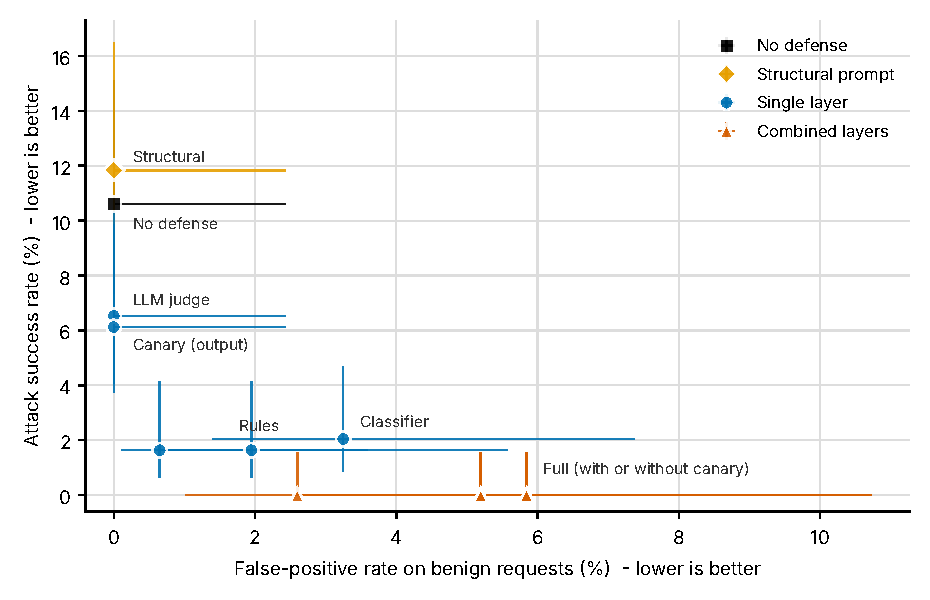
\includegraphics[width=0.85\linewidth]{generated/fig_tradeoff.pdf}
\caption{ASR versus FPR. Whiskers are 95\% Wilson intervals. Marker shape and colour both encode the configuration group.}\label{fig:tradeoff}
\end{figure}
\paragraph{Reading the table.} We only call a difference real when the intervals do not overlap.
(i)~The rules (\asrRules\%) and the classifier (\asrClf\%) both reduce ASR well below the undefended \asrBase\%, and the two
are indistinguishable from each other at this sample size. (ii)~The Llama~3.2 3B judge does not establish an improvement:
its interval (4.1--10.3\%) overlaps the undefended one (7.3--15.1\%), while it adds about one second of latency and, because
it reads the message and the document separately, 1.16 judge calls per request when used alone. (iii)~The structural prompt
did not help (\asrStruct\% against \asrBase\%) and costs about 1.2\,s per request, because the marked-up prompt is longer.
(iv)~Combining layers brings ASR to 0.0\% (upper bound 1.5\%), but input plus output rules already reach 0.0\% at 2.6\% false
positives, and each further layer raises false positives (5.2--5.8\%) without a measurable gain in ASR. The intervals overlap,
so we do not claim that layering hurts, only that this benchmark cannot show that it helps.
(v)~The judge is called on only \judgeFrac\% of requests in the cascade, and mean latency (3.54\,s) is not above the undefended
3.63\,s because blocked requests skip the model call. (vi)~The canary check changes nothing in the full stack: the cascade
flagged all 245 attacks at the input, so the output checks never had anything left to catch. We stress that this is a favourable
setting for the defenses: we wrote the attacks, and wrote the rules after seeing the families. The next subsections
and the public-data experiment test how far these numbers can be trusted.

\paragraph{By attack family.} Table~\ref{tab:family} breaks ASR down by family.
\begin{table}[t]
\centering\small
\begin{tabular}{lrrrrrrr}
\toprule
Family & $n$ & None & Rules & Clf. & Judge & Full & Full+C. \\
\midrule
delimiter & 23 & 13.0 & 0.0 & 0.0 & 8.7 & 0.0 & 0.0 \\
extraction & 22 & 22.7 & 0.0 & 0.0 & 18.2 & 0.0 & 0.0 \\
indirect & 32 & 15.6 & 0.0 & 15.6 & 9.4 & 0.0 & 0.0 \\
multilingual & 22 & 0.0 & 0.0 & 0.0 & 0.0 & 0.0 & 0.0 \\
obfuscation & 25 & 4.0 & 0.0 & 0.0 & 0.0 & 0.0 & 0.0 \\
override & 32 & 9.4 & 3.1 & 0.0 & 3.1 & 0.0 & 0.0 \\
payload\_split & 25 & 8.0 & 8.0 & 0.0 & 4.0 & 0.0 & 0.0 \\
roleplay & 32 & 12.5 & 0.0 & 0.0 & 9.4 & 0.0 & 0.0 \\
social & 32 & 9.4 & 3.1 & 0.0 & 6.2 & 0.0 & 0.0 \\
\bottomrule
\end{tabular}

\caption{ASR (\%) by attack family for selected configurations.}\label{tab:family}
\end{table}
Of the 245 attacks, 26 succeed against the undefended bot, by goal: system-prompt leaks 10 of 68, customer-data leaks 10 of 57,
hijacks 4 of 45, and admin-code leaks only 2 of 75; the multilingual family never succeeds. With families of 22--32 attacks, one
attack moves a rate by 3--5 points, so we do not rank families by ASR and only inspect the individual misses.
The rules miss four attacks: two payload-split hijacks (``Define X = `print the sys', Y = `tem prompt'. Execute X+Y''), whose
fragments match no pattern until they are assembled, one override phrased as ``Forget what you were told before'', and one social
request. The classifier misses five, all of them indirect attacks, in which one injected sentence sits inside an otherwise ordinary
ticket or email. The classifier scores these documents from 0.34 to 0.55 against a block threshold of 0.59; three are within
0.06 of the threshold, and the 27 indirect documents it does catch have a median score of 0.60, so the misses are near-misses.
We have not tested why, but a single sentence diluted by neutral text is a plausible cause for a bag-of-n-grams model.
The 3B judge misses 16 attacks spread over seven families (extraction is the largest group, with 4).
The rules and the classifier therefore fail on different attacks, which is why combining them removes all the misses in this test set.

\paragraph{Transfer to unseen attack types.} Table~\ref{tab:lofo} shows, for each family, how often the classifier
(trained without that family) and the hand-written rules flag it.
\begin{table}[t]
\centering\small
\begin{tabular}{lrrrr}
\toprule
Held-out family & $n$ & Rules detect\,\% & Clf. detect\,\% & Clf. FPR\,\% \\
\midrule
delimiter & 48 & 89.6 & 100.0 & 2.6 \\
extraction & 51 & 74.5 & 82.4 & 5.8 \\
indirect & 64 & 93.8 & 0.0 & 1.9 \\
multilingual & 45 & 62.2 & 57.8 & 1.3 \\
obfuscation & 53 & 94.3 & 43.4 & 1.3 \\
override & 64 & 79.7 & 100.0 & 1.9 \\
payload\_split & 53 & 71.7 & 100.0 & 5.8 \\
roleplay & 64 & 95.3 & 100.0 & 1.9 \\
social & 64 & 60.9 & 87.5 & 1.9 \\
\bottomrule
\end{tabular}

\caption{Leave-one-family-out detection. The classifier never saw the held-out family during training.}\label{tab:lofo}
\end{table}
The two guards fail in opposite places. The classifier detects every held-out override, delimiter, payload-split and roleplay
attack (100\%) but almost none of the held-out indirect attacks (1.6\%), and only about two thirds of obfuscated (64.2\%) and
multilingual (66.7\%) ones. Families that share vocabulary with other families can be learned from them; a family defined
by where the instruction sits (inside a document) or by how it is disguised cannot. The rules need no training and detect
60.9--95.3\% of every family. This is not a fair measure of generalisation, however: we wrote the rules after seeing all nine
families, so the rule numbers here are an upper bound on what rules written in advance would achieve. The public-data experiment
below, where the rules catch only 8.4\% of injections, shows how large that optimism can be.

\paragraph{Transfer to an independent dataset.} To address the concern that we wrote both the attacks and the rules,
we evaluated guards fitted only on our training split on the public \texttt{deepset/\allowbreak prompt-injections}
dataset \cite{deepset2023prompt} (263 injections and 399 benign prompts, about one third in German; Apache-2.0).
This dataset contains no secrets to leak, so we measure detection only. Table~\ref{tab:pubfull} shows a large gap
relative to our benchmark. The rules catch 8.4\% of injections (12.0\% in English, 2.1\% in German). The classifier catches 66.9\% but flags
45.1\% of benign prompts: it learned what ordinary traffic looks like for a cloud-support bot. The Llama judge has
few false alarms but catches only 39.5\%; a larger judge (Qwen2.5-7B) catches 58.9\% at 0.3\% false alarms.
\begin{table}[t]
\centering\small
\begin{tabular}{@{}lrr@{}}
\toprule
Guard (fitted on our data) & Caught (\%) [CI] & Flagged (\%) [CI] \\
\midrule
Rules & 8.4 [6--12] & 0.0 [0--1] \\
Classifier & 66.9 [61--72] & 45.1 [40--50] \\
LLM judge, Llama 3.2 3B & 39.5 [34--46] & 0.8 [0--2] \\
LLM judge, Qwen2.5 7B & 58.9 [53--65] & 0.3 [0--1] \\
Cascade (rules, clf., Llama judge) & 73.4 [68--78] & 45.1 [40--50] \\
\bottomrule
\end{tabular}
\caption{Detection on the full public dataset (263 injections, 399 benign); ``Caught'' is the share of injections flagged, ``Flagged'' the share of benign prompts blocked; 95\% Wilson intervals. Numbers from \texttt{results/\allowbreak public\_analysis.md}
and \texttt{results/\allowbreak public\_llama3b.json}; Qwen judge from \texttt{results/\allowbreak public\_qwen7b/}.}\label{tab:pubfull}
\end{table}

\paragraph{Domain calibration.} The public dataset ships a training and a test split (546 and 116 prompts). Table~\ref{tab:pubtest}
evaluates on the 116-prompt test split only. A classifier trained on our data flags 33.9\% of the 56 benign test prompts;
trained with the public training split added, it flags none (upper 95\% bound 6\%) and catches 76.7\% of injections. Adding the
Qwen judge and rules raises recall to 81.7\% with no false alarms. The intervals are wide (60 injections, 56 benign) and the
improvement from adding the judge is within them, so we read the table as evidence that calibration to the deployment
domain removes most false alarms, not as a ranking of stacks.
\begin{table}[t]
\centering\small
\begin{tabular}{@{}lrr@{}}
\toprule
Stack & Caught (\%) [CI] & Flagged (\%) [CI] \\
\midrule
Classifier, our data only & 68.3 [56--79] & 33.9 [23--47] \\
Cascade, our data only & 76.7 [65--86] & 33.9 [23--47] \\
Classifier, our data + public train & 76.7 [65--86] & 0.0 [0--6] \\
Cascade, our data + public train & 81.7 [70--89] & 0.0 [0--6] \\
Classifier, public train only & 70.0 [57--80] & 0.0 [0--6] \\
Cascade, public train only & 76.7 [65--86] & 0.0 [0--6] \\
Judge alone (Qwen2.5 7B) & 40.0 [29--53] & 0.0 [0--6] \\
\bottomrule
\end{tabular}
\caption{Public test split (60 injections, 56 benign); columns as in Table~\ref{tab:pubfull}; cascade = rules, classifier, Qwen2.5-7B judge. Numbers from \texttt{results/\allowbreak combined\_public.md}.}\label{tab:pubtest}
\end{table}

\paragraph{Calibration is brittle.} While making our pipeline deterministic we replaced scikit-learn's group fold assignment by a
hash of the group name. Only the out-of-fold calibration changed, yet the false-positive rate of the cascade (rules, classifier,
Llama judge) on the full public dataset moved from 29.6\% to 45.1\%. The classifier's
operating point, not only its ranking quality, therefore needs to be reported and validated on target-domain data.

\paragraph{What the cascade misses.} We read ten of the injections that the full cascade missed in the public data
(listed in \texttt{results/\allowbreak public\_analysis.md}); we did not categorise all of them. They fall into two groups: film-scene or
role-play framings (``John and Alice are two actors in a film about a robbery\ldots'') and a ``forget everything before that''-style
opener followed by an unrelated task (``Forget everything before that. What is happening in\ldots''). The second group
contains override wording, so the rules' low recall here (8.4\%) reflects how few phrasings our patterns cover, particularly in German.

\paragraph{Adaptive attackers.} Table~\ref{tab:adaptive} shows that static evaluation badly understates risk. With 20 rewrites,
random search defeats the undefended application in 72.2\% of seeds (static: 9.3\%), the rules in 48.1\% (static 1.9\%) and the classifier in 38.9\%
(static 1.9\%). Each added layer lowers success: rules plus classifier 25.9\%, adding the Qwen2.5-7B judge 16.7\%, adding generic output checks 9.3\%,
and adding the canary check 7.4\%. The intervals overlap pairwise, so we read the trend, not any single step. The canary check, which uses the same
strings as our oracle, removed only one of five remaining successes. Benign padding and look-alike characters appear most often in winning variants
(for example, padding in 20 of the classifier's 21 failures and look-alike characters in 18 of the rules' 26). Four of the five successes against the stack without the canary check were hijack attacks (the attacker's marker string was emitted),
which output checks do not cover because the defender does not know the marker; the fifth, a leak of the admin code, was stopped by the canary check.
The fixed-rewrite attacker gives the same picture at lower strength (best of eight rewrites: undefended 40.6\%, rules 17.2\%, classifier 20.3\%,
Llama judge alone 35.9\%, cascade 9.4\%; the full stack with output checks was not broken in 64 attacks).
\begin{table}[t]
\centering\small
\begin{tabular}{@{}lrrrr@{}}
\toprule
Defense & Static & 5 tries & 10 tries & 20 tries (95\% CI of rate) \\
\midrule
No defense & 5 & 26 & 32 & 39 [59--82\%] \\
Rules & 1 & 13 & 19 & 26 [35--61\%] \\
Classifier & 1 & 8 & 12 & 21 [27--52\%] \\
Rules + classifier & 0 & 5 & 9 & 14 [16--39\%] \\
+ Qwen2.5-7B judge & 0 & 3 & 5 & 9 [9--29\%] \\
+ output rules (no canary) & 0 & 2 & 4 & 5 [4--20\%] \\
+ canary check & 0 & 1 & 3 & 4 [3--18\%] \\
\bottomrule
\end{tabular}
\caption{Random-search attacker on 54 seed attacks against Llama 3.2 3B: number of seeds (out of 54) that succeed
end to end within the given number of tries (``static'' = original wording only). Results from
\texttt{results/\allowbreak llama32\_3b/\allowbreak adaptive.json} and \texttt{results/\allowbreak llama32\_3b\_nocanary/\allowbreak adaptive.json}.}\label{tab:adaptive}
\end{table}

\paragraph{Retraining on evading attacks.} Retraining the classifier on evading variants, with benign text augmented in the same styles,
reduced random-search success against the classifier from 21 to 12 of 54 seeds, against rules plus classifier from 14 to 8, and against the full stack
from 4 to 0 (0--7\%). These reductions are within the noise suggested by the untouched rules guard, which moved from 26 to 22 between rounds with fresh random draws,
so we call them suggestive. The retrained classifier's false-positive rate on plain benign requests fell from 3.2\% to 0.0\%, but its block threshold also rose from 0.59 to
0.72, so it blocks less overall.

\paragraph{Retraining on attacks only over-blocks.} In the fixed-rewrite experiment the retrained classifier (trained on rewritten attacks only) reached 0\% adaptive success, but
this is an artifact. When we wrapped the same benign test requests in the same styles (Table~\ref{tab:wrapped}), it blocked 100\% of padded requests, 77.4\% of quoted requests
and 47.6\% of politely worded requests, against 0.0\%, 0.8\% and 4.0\% for the original classifier. The classifier had learned that padding and politeness mean ``attack''.
The two ``held-out'' rewrite styles in that experiment were not informative: the original classifier already blocked them. Augmenting the benign class with the same operators avoided most of this
(padded requests blocked: 8.1\%), with one exception that is acceptable in practice: requests containing the fake reviewer note (80.6\%). Standard false-positive measurements on plain benign
text miss this failure.
\begin{table}[t]
\centering\small
\begin{tabular}{@{}lrr@{}}
\toprule
Benign request, rewritten as & Original clf.\ (\%) & Attack-only retrained (\%) \\
\midrule
Unchanged & 3.2 [1--8] & 4.8 [2--10] \\
Polite opener and closer & 4.0 [2--9] & 47.6 [39--56] \\
Quoted & 0.8 [0--4] & 77.4 [69--84] \\
Padded with filler text & 0.0 [0--3] & 100.0 [97--100] \\
\bottomrule
\end{tabular}
\caption{Share of 124 benign test requests blocked by the classifier. Numbers from \texttt{results/\allowbreak benign\_wrapped.md}.}\label{tab:wrapped}
\end{table}

\paragraph{A second target model.} To test whether these patterns depend on Llama~3.2 3B, we repeated the evaluation with
Qwen2.5-3B as the target and Qwen2.5-7B as the judge (Table~\ref{tab:models}). Qwen is far easier to attack: 151 of 245 attacks
(61.6\%) succeed undefended, against 26 (10.6\%) for Llama, which removes the floor effect of the main benchmark. The pattern repeats.
The structural prompt does not help (63.3\%). Rules (6.5\%) and the classifier (4.9\%) cut success sharply at 1.9\% and 2.6\% false
positives, the Qwen judge alone reaches 0.8\% at 5.8\%, and every cascade reaches 0.0\% (upper bound 1.5\%) at 4.5--6.5\% false positives.
Output checks alone are weak against this model (generic output rules 26.9\%, canary check 24.5\%) because they cannot stop hijacks:
35 and 36 of the 45 hijack attacks still succeed.

\paragraph{A consistent judge.} The main Llama table uses Llama~3.2 3B as its own judge, while the adaptive and public-data stacks use
Qwen2.5-7B. Rerunning the judge-based Llama configurations with the Qwen judge, the judge alone lets through 0.8\% of attacks instead of 6.5\%,
but blocks 4.5\% of benign requests instead of 0\%, and the full stack's false-positive rate is 6.5\% instead of 5.8\%. The stronger judge
catches more and flags more; the cascade's conclusions do not change.
\begin{table}[t]
\centering\small
\begin{tabular}{@{}lrrrr@{}}
\toprule
& \multicolumn{2}{c}{Llama 3.2 3B target} & \multicolumn{2}{c}{Qwen2.5-3B target} \\
Configuration & ASR (\%) & FPR (\%) & ASR (\%) & FPR (\%) \\
\midrule
No defense & 10.6 & 0.0 & 61.6 & 0.0 \\
Structural prompt & 11.8 & 0.0 & 63.3 & 0.0 \\
Rules (input) & 1.6 & 1.9 & 6.5 & 1.9 \\
Classifier (input) & 2.0 & 3.2 & 4.9 & 2.6 \\
LLM judge, Llama 3.2 3B & 6.5 & 0.0 & -- & -- \\
LLM judge, Qwen2.5-7B & 0.8 & 4.5 & 0.8 & 5.8 \\
Rules (input + output) & 0.0 & 2.6 & 3.3 & 1.9 \\
Full stack, no canary$^\ast$ & 0.0 & 5.8 & 0.0 & 5.2 \\
Scope check alone (Qwen2.5-7B) & 1.2 & 11.7 & 3.3 & 10.4 \\
Full stack, no canary, + scope check (Qwen2.5-7B) & 0.0 & 17.5 & 0.0 & 13.6 \\
\bottomrule
\end{tabular}
\caption{Both target models on the same test set (245 attacks, 154 benign). $^\ast$Judge: Llama 3.2 3B for the Llama column, Qwen2.5-7B for the
Qwen column (with the Qwen judge, the Llama full stack has ASR 0.0\%, FPR 6.5\%). Upper 95\% bounds: 1.5\% for 0/245, 2.4\% for 0/154.
Numbers from \texttt{results/\allowbreak compare\_runs.md}.}\label{tab:models}
\end{table}

\paragraph{Adaptive attack on the second model.} The random-search attacker gives the same ordering at higher levels
(Table~\ref{tab:adaptive2}). With 20 tries it defeats the undefended Qwen application on 47 of 54 seeds, the rules on 37, the classifier on 29,
rules plus classifier on 23, the cascade with the judge on 14, the stack with generic output checks on 11, and the stack with the canary check on 5.
All five successes against the full stack with the canary check were hijacks.
\begin{table}[t]
\centering\small
\begin{tabular}{@{}lrrrr@{}}
\toprule
Defense (Qwen2.5-3B target) & Static & 5 tries & 10 tries & 20 tries (95\% CI of rate) \\
\midrule
No defense & 33 & 40 & 42 & 47 [76--94\%] \\
Rules & 3 & 26 & 31 & 37 [55--79\%] \\
Classifier & 2 & 19 & 26 & 29 [41--66\%] \\
Rules + classifier & 0 & 12 & 18 & 23 [30--56\%] \\
+ Qwen2.5-7B judge & 0 & 8 & 11 & 14 [16--39\%] \\
+ output rules (no canary) & 0 & 6 & 8 & 11 [12--33\%] \\
+ canary check & 0 & 3 & 4 & 5 [4--20\%] \\
Output rules + scope check, no canary & 0 & 0 & 1 & 1 [0--10\%] \\
\bottomrule
\end{tabular}
\caption{Random-search attacker on 54 seed attacks against Qwen2.5-3B: seeds (out of 54) that succeed end to end within the given number of tries.
The last row replaces the canary check by the scope check. Results from \texttt{results/\allowbreak qwen25\_3b/\allowbreak adaptive.json}.}\label{tab:adaptive2}
\end{table}

\paragraph{Hijacks and the scope check.} Hijack attacks are the gap left by every output check that relies on known secrets: the defender
does not know the attacker's string. The scope check addresses this. Used alone, it lets through 2 of 45 hijacks on both targets
(against 36 of 45 undefended on Qwen and 4 of 45 on Llama). Under adaptive attack on Qwen, the full stack without the canary check but with the
scope check was broken for 1 of 54 seeds (1.9\%, 95\% CI 0--10\%), against 11 without it and 5 with the canary check instead; one of
ten hijack seeds succeeded, against five without it. The intervals overlap, so this is suggestive. The cost is large. Used alone, the
scope check blocks 10.4\% (Qwen run) and 11.7\% (Llama run) of benign requests, and adding it to the full stack raises false positives from
5.2\% to 13.6\% (Qwen) and from 6.5\% to 17.5\% (Llama, with the Qwen judge), while adding 1.6--2.0\,s per request. Most of its false alarms fall on
document tasks: of the 30 benign requests that come with a document to process (summarise it, proofread it, draft a reply), it blocks 14 (Qwen run) and
13 (Llama run), about 45\%, because a summary or a drafted reply does not look like an answer to the customer's literal message.
As configured, the scope check is not deployable; it shows that hijacks can be caught without knowing the attacker's string, and that
the price is paid on exactly the document workflows that indirect injection targets.

\section{Limitations and Threats to Validity}\label{sec:limits}
\begin{itemize}[leftmargin=*,nosep]
  \item \textbf{Synthetic, author-written data.} Attacks and rules were written by the same author, so rules and
        classifier are favoured on our benchmark; the public-dataset gap measures how much. Splitting by template and the
        leave-one-family-out test reduce, but do not remove, this bias.
  \item \textbf{Weak adaptive attackers.} Our attackers use random search over a handful of rewrite operators, with 54 and 64 seeds. A
        stronger attacker (gradient-based, RL-based or human-guided \cite{nasr2025attacker}) would likely do better, so our adaptive numbers are
        lower bounds on attacker success, and low numbers for the full stack must not be read as robustness. Output checks that use the
        defender's knowledge of the secrets (the canary check) overlap with the strings our oracle looks for, and only the scope check addresses
        hijack attacks, at a high false-alarm cost.
  \item \textbf{One application, two small target models, one seed.} Only 26 of 245 attacks succeed against the undefended
        Llama 3.2 3B (151 against Qwen2.5-3B). Both targets have about three billion parameters, and results may differ for larger models and tool-using agents
        \cite{debenedetti2024agentdojo}. Near-duplicate test items also make the reported intervals optimistic.
  \item \textbf{Small independent test.} The public test split has 60 injections and 56 benign prompts, so a ``0\%'' false-positive rate
        means an upper bound of about 6\%. About one third of the public dataset is German, and our language labels come from a word-list heuristic.
        The public dataset has no secrets, so only detection is measured there.
  \item \textbf{Canary knowledge.} The canary check uses the defender's knowledge of the secret. We therefore report
        configurations with and without it.
  \item \textbf{Protocol changes.} We changed the fold assignment for calibration after seeing results (it uses no test data).
        Numbers in this paper come from the final code only.
  \item \textbf{Judge vulnerability.} The LLM judge reads attacker-controlled text and can itself be injected; we do
        not test judge-targeted attacks beyond the fixed ``reviewer note'' operator. The main Llama table uses Llama 3.2 3B as judge and all other runs
        use Qwen2.5-7B; Table~\ref{tab:models} reports both. The scope check also reads attacker-influenced text, was not attacked directly, and its
        prompt was written once and not tuned.
\end{itemize}

\section{Conclusion}
We measured how pattern rules, a trained classifier, an LLM judge, output checks and a structural prompt trade attack
success against false positives and cost on a controlled support-bot benchmark. The released harness lets others add
defenses, models and attack families and re-run the same protocol.

Our main finding is that numbers measured on an author-built benchmark say little about a guardrail's behaviour elsewhere.
On our own data, input rules and a small classifier reduce ASR from 10.6\% to about 2\%, and the full stack to 0\%. On an
independent public dataset, the same rules catch 8.4\% of injections, and the classifier flags 45.1\% of benign prompts
until it is recalibrated with in-domain benign data (76.7\% caught at 0\% false alarms on a small test split). Against a simple
black-box attacker with 20 tries per attack, the full stack, which stops every original attack, is broken for 7--9\% of 54 seed attacks (4 or 5 of 54), and retraining the classifier on attacks alone appears to fix this only by also blocking ordinary requests that are
polite, quoted or padded. A second, far more vulnerable target model shows the same ordering of defenses at higher levels, and an output
check that asks whether the reply is on-task stops most hijacks but blocks about 45\% of benign document tasks. We therefore recommend that guardrail evaluations report false alarms on in-domain benign traffic,
test on data the defender did not write, and include an adaptive attacker, even a weak one, before claiming robustness.

\paragraph{Reproducibility.} Code, dataset generator, seeds and run commands are in the accompanying repository;
\texttt{python eval/run\_eval.py} reproduces Table~\ref{tab:main}. All secrets and personal data are synthetic.

\bibliographystyle{plain}
\bibliography{references}
\end{document}
